\section{Definição}

\begin{frame}[fragile]{Listas encadeadas}

    \begin{itemize}
        \item Uma lista encadeada, ou simplesmente lista, é uma estrutura composta por nós,
            onde cada nó armazenada uma informação e um ponteiro para o próximo nó da lista

        \item Conhecido o primeiro elemento da lista (\textit{head}), é possível acessar todos
            os demais elementos

        \item Uma lista é uma estrutura de dados linear, devido a travessia sequencial e ordenada
            de seus elementos

        \item As listas são uma alternativa aos vetores: a vantagem do acesso aleatório imediato dos
            vetores é substituída pela inserção e remoção eficientes

        \item Por conta da estrutura dos nós, o acesso aleatório em listas encadeadas tem
            complexidade $O(N)$

    \end{itemize}

\end{frame}

\begin{frame}[fragile]{Visualização de uma lista encadeada}

    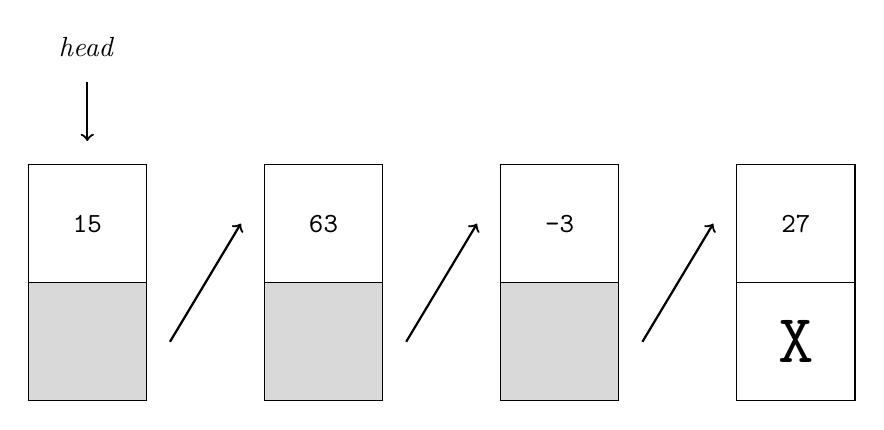
\begin{tikzpicture}[scale=1.5]
        \node[anchor=center] at (0.5, 3) {\textit{head}};
        \draw[->,thick] (0.5, 2.7) -- (0.5, 2.2);

        \draw[fill=white] (0,1) rectangle (1,2);
        \draw[fill=gray!30] (0,0) rectangle (1,1);
        \node at (0.5,1.5) {\texttt{15}};

        \draw[->,thick] (1.2, 0.5) -- (1.8, 1.5);
        \draw[fill=white] (2,1) rectangle (3,2);
        \draw[fill=gray!30] (2,0) rectangle (3,1);
        \node at (2.5,1.5) {\texttt{63}};

        \draw[->,thick] (3.2, 0.5) -- (3.8, 1.5);
        \draw[fill=white] (4,1) rectangle (5,2);
        \draw[fill=gray!30] (4,0) rectangle (5,1);
        \node at (4.5,1.5) {\texttt{-3}};

        \draw[->,thick] (5.2, 0.5) -- (5.8, 1.5);
        \draw[fill=white] (6,1) rectangle (7,2);
        \draw (6,0) rectangle (7,1);
        \node at (6.5,1.5) {\texttt{27}};
        \node at (6.5,0.5) {\Huge \textbf{\texttt{X}}};

    \end{tikzpicture}

\end{frame}

\begin{frame}[fragile]{Implementação de uma lista encadeada}

    \begin{itemize}
        \item Uma lista pode ser implementada como uma \code{c}{struct} em C ou uma
            classe em C++

        \item A lista deve ter, no mínimo, um membro para o primeiro elemento da lista
            (\textit{head})

        \item Cada nó deve ter, no mínimo, dois membro: um para armazenar as informações 
            (\code{c}{info}) e outro para representar o ponteito para o próximo nó
            (\code{c}{next})

        \item O último elemento da lista tem membro \code{c}{next} nulo

        \item A adição de um ponteiro para o último elemento da lista (\textit{tail}) aumenta
            a memória usada pela lista, mas permite a inserção ao final em complexidade $O(1)$
    \end{itemize}

\end{frame}

\begin{frame}[fragile]{Exemplo de implementação de uma lista encadeada}
    \inputsnippet{cpp}{1}{20}{list.h}
\end{frame}

\begin{frame}[fragile]{Exemplo de implementação de uma lista encadeada}
    \inputsnippet{cpp}{21}{40}{list.h}
\end{frame}

\begin{frame}[fragile]{Exemplo de implementação de uma lista encadeada}
    \inputsnippet{cpp}{90}{110}{list.h}
\end{frame}

